\documentclass[a4paper,12pt]{article}
\usepackage[utf8]{inputenc}
\usepackage{graphicx}
\usepackage{parskip}
\usepackage{float}

\linespread{1.2}
\newenvironment{itenv}
{\itshape}
    {}

\title{New Zealand's policy to combat Climate Change}
\author{\vspace{-8ex}}
\date{\vspace{-8ex}}

\begin{document}

\maketitle

Word count: 791\\
Article: https://www.theguardian.com/environment/2021/jun/14/new-zealand-unveils-8600-subsidy-for-electric-vehicles-to-reduce-emissions, ``New Zealand unveils \$8,600 subsidy for electric vehicles to reduce emissions'', published by the Guardian, written by Tess McClure on 14/07/2021, accessed 23/08/2021\\
Topic: Microeconomics\\
Key Concept: Intervention

\newpage
\section*{Article}
\begin{itenv}
New Zealand unveils \$8,600 subsidy for electric vehicles to reduce emissions

Move comes after Climate Commission recommended banning petrol and diesel cars by 2023
\end{itenv}


The New Zealand government is introducing subsidies to make electric vehicles thousands of dollars cheaper and new petrol and diesel cars more expensive, as the country tries transition to an emissions-free fleet.

The changes follow New Zealand’s Climate Commission recommendations which laid out sweeping changes required to get the country closer to its emissions targets.

The subsidies for electric and some hybrid vehicles would be up to NZ\$8,625 (£4,360) for new vehicles and NZ\$3,450 (£1,744) for used cars. They will start next month.

Transport now makes up almost 33\% of long-lived greenhouse gas emissions in Aotearoa, and last week, the Climate Commission laid out new benchmarks for the country to transform the makeup of its fleet. The commission’s recommended plan included banning imports of petrol and diesel cars by 2032, and that road transport be almost completely decarbonised by 2050. To meet its goal for transport emissions, the commission concluded electric vehicles would need to make up half of all light vehicle registrations by 2029, and 100\% by 2035.

“Our transport emissions are the fastest growing source of greenhouse gas emissions in New Zealand, so we need to start taking action now if we are going to meet our 2050 targets,” transport minister Michael Wood said in a written statement.

“New Zealand is actually lagging behind on the uptake of EVs, so we are playing catch up internationally,” he said. He said the policy would prevent up to an estimated 9.2m tonnes of carbon dioxide emissions.

The subsidies would be funded by introducing new charges on imports of high-emission utility vehicles and SUVs. For example, an imported Toyota Hilux – one of New Zealand’s more popular utes – could incur a fee of NZ\$2,900. Those fees would kick in at the start of January 2022.

New Zealand is one of the world’s worst performers on emission increases, and hitting its climate goals will require a reversal of its current trajectory. The country’s emissions rose by 57\% between 1990 and 2018 – the second greatest increase of all industrialised countries. Earlier this year, data showed that New Zealand’s emissions had increased by 2\% in 2018-19.

Climate change minister James Shaw said that at present, low emissions vehicles were financially out of the reach of many New Zealanders.

“As technology develops and more manufacturers decide to stop making petrol and diesel cars, the cost of low emissions vehicles will come down. However at the moment they are still more expensive to buy. Today’s announcement helps to address that,” he said.

The policy has sparked some criticism. Centre-right opposition party National said tying the rebates to fees on higher-emissions vehicles meant it amounted to a “reverse Robin Hood” strategy – imposing fees on lower and middle-income New Zealanders while subsidising those wealthy enough to afford a new electric vehicle. The policy would “unfairly hurt farmers, tradespeople and low-income earners for whom low-emission vehicles will still be too expensive or unsuitable for their lifestyle,” said shadow transport spokesperson Michael Woodhouse.

Woodhouse said National supported incentives for people to buy EVs but disagreed with financially punishing those who didn’t.

Wood said that the policy “only applies to new and used cars arriving in New Zealand, so the existing secondhand market of cars that lower income families tend to purchase from will not be affected”.

Shaw said the policy “will also stimulate the second-hand market, so in the years to come even more people can access low carbon transport options”.

Many other nations already have subsidies for electric vehicles. Germany introduced a €4,000 (NZ\$6,785) subsidy for electric vehicles back in 2016. Slightly less-generous subsidies exist in the UK, where buyers can get a grant for an electric cars of £2,500 (nearly NZ\$5,000) – reduced from £3,000 in March.

Other countries have taken more radical steps. In Norway, electric cars now make up 54\% of market share, after the country exempted fully electric vehicles from taxes imposed on those relying on fossil fuels. That move made new electric models cheaper than some comparable petrol cars for Norwegians.

\newpage

\section*{Topic}
The article chosen discussed the New Zealand government's plan to subsidize the electric vehicles (EV) market. The country is falling behind in reaching its climate goals of lower emissions --- a net-zero emission by 2050. Thus it is proposing a subsidy in the form of rebates for new EV purchased of up to NZ\$8,625 per unit. The policy aims to increase the saturation of EVs in market, and attempt to decrease the negative externality of consumption with gasoline vehicles of its environmental damages. We will focus on \textbf{intervention}, its impacts, and justifications for the action.

% key concept
%Intervention is the key concept in focus, because the article is a description of an government intervention in the forms of a subsidy. Theories will be constructed to analyze the subsidy, and we will be evaluating its implications. The idea of intervention will be touched on throughout the text.

\section*{Theory}

% model, explaination
The government intervened in the EV market with a subsidy on the purchase of newly produced electric vehicles. Figure \ref{fig:sub} shows the effect of the \textbf{intervention} on the EV market. The subsidy, paid by the government per unit purchase to the consumers, will decrease the cost of buying for consumers. The demand curve will shift upwards --- for consumers are more able to buy, from $D_1$ to $D_2$, the amount of the subsidy. A shortage will occur, consumers will bid up the price in fear of missing out. This causes the equilibrium to shift from $A$ to $B$, increasing quantity demanded of EVs from $Q_1$ to $Q_2$ and increasing the price from $P_1$ to $P_2$. The cost of the subsidy is $P_2BCP_0$, and creating a dead-weight loss (DWL) of size $ABC$.

\begin{figure}
    \centering
    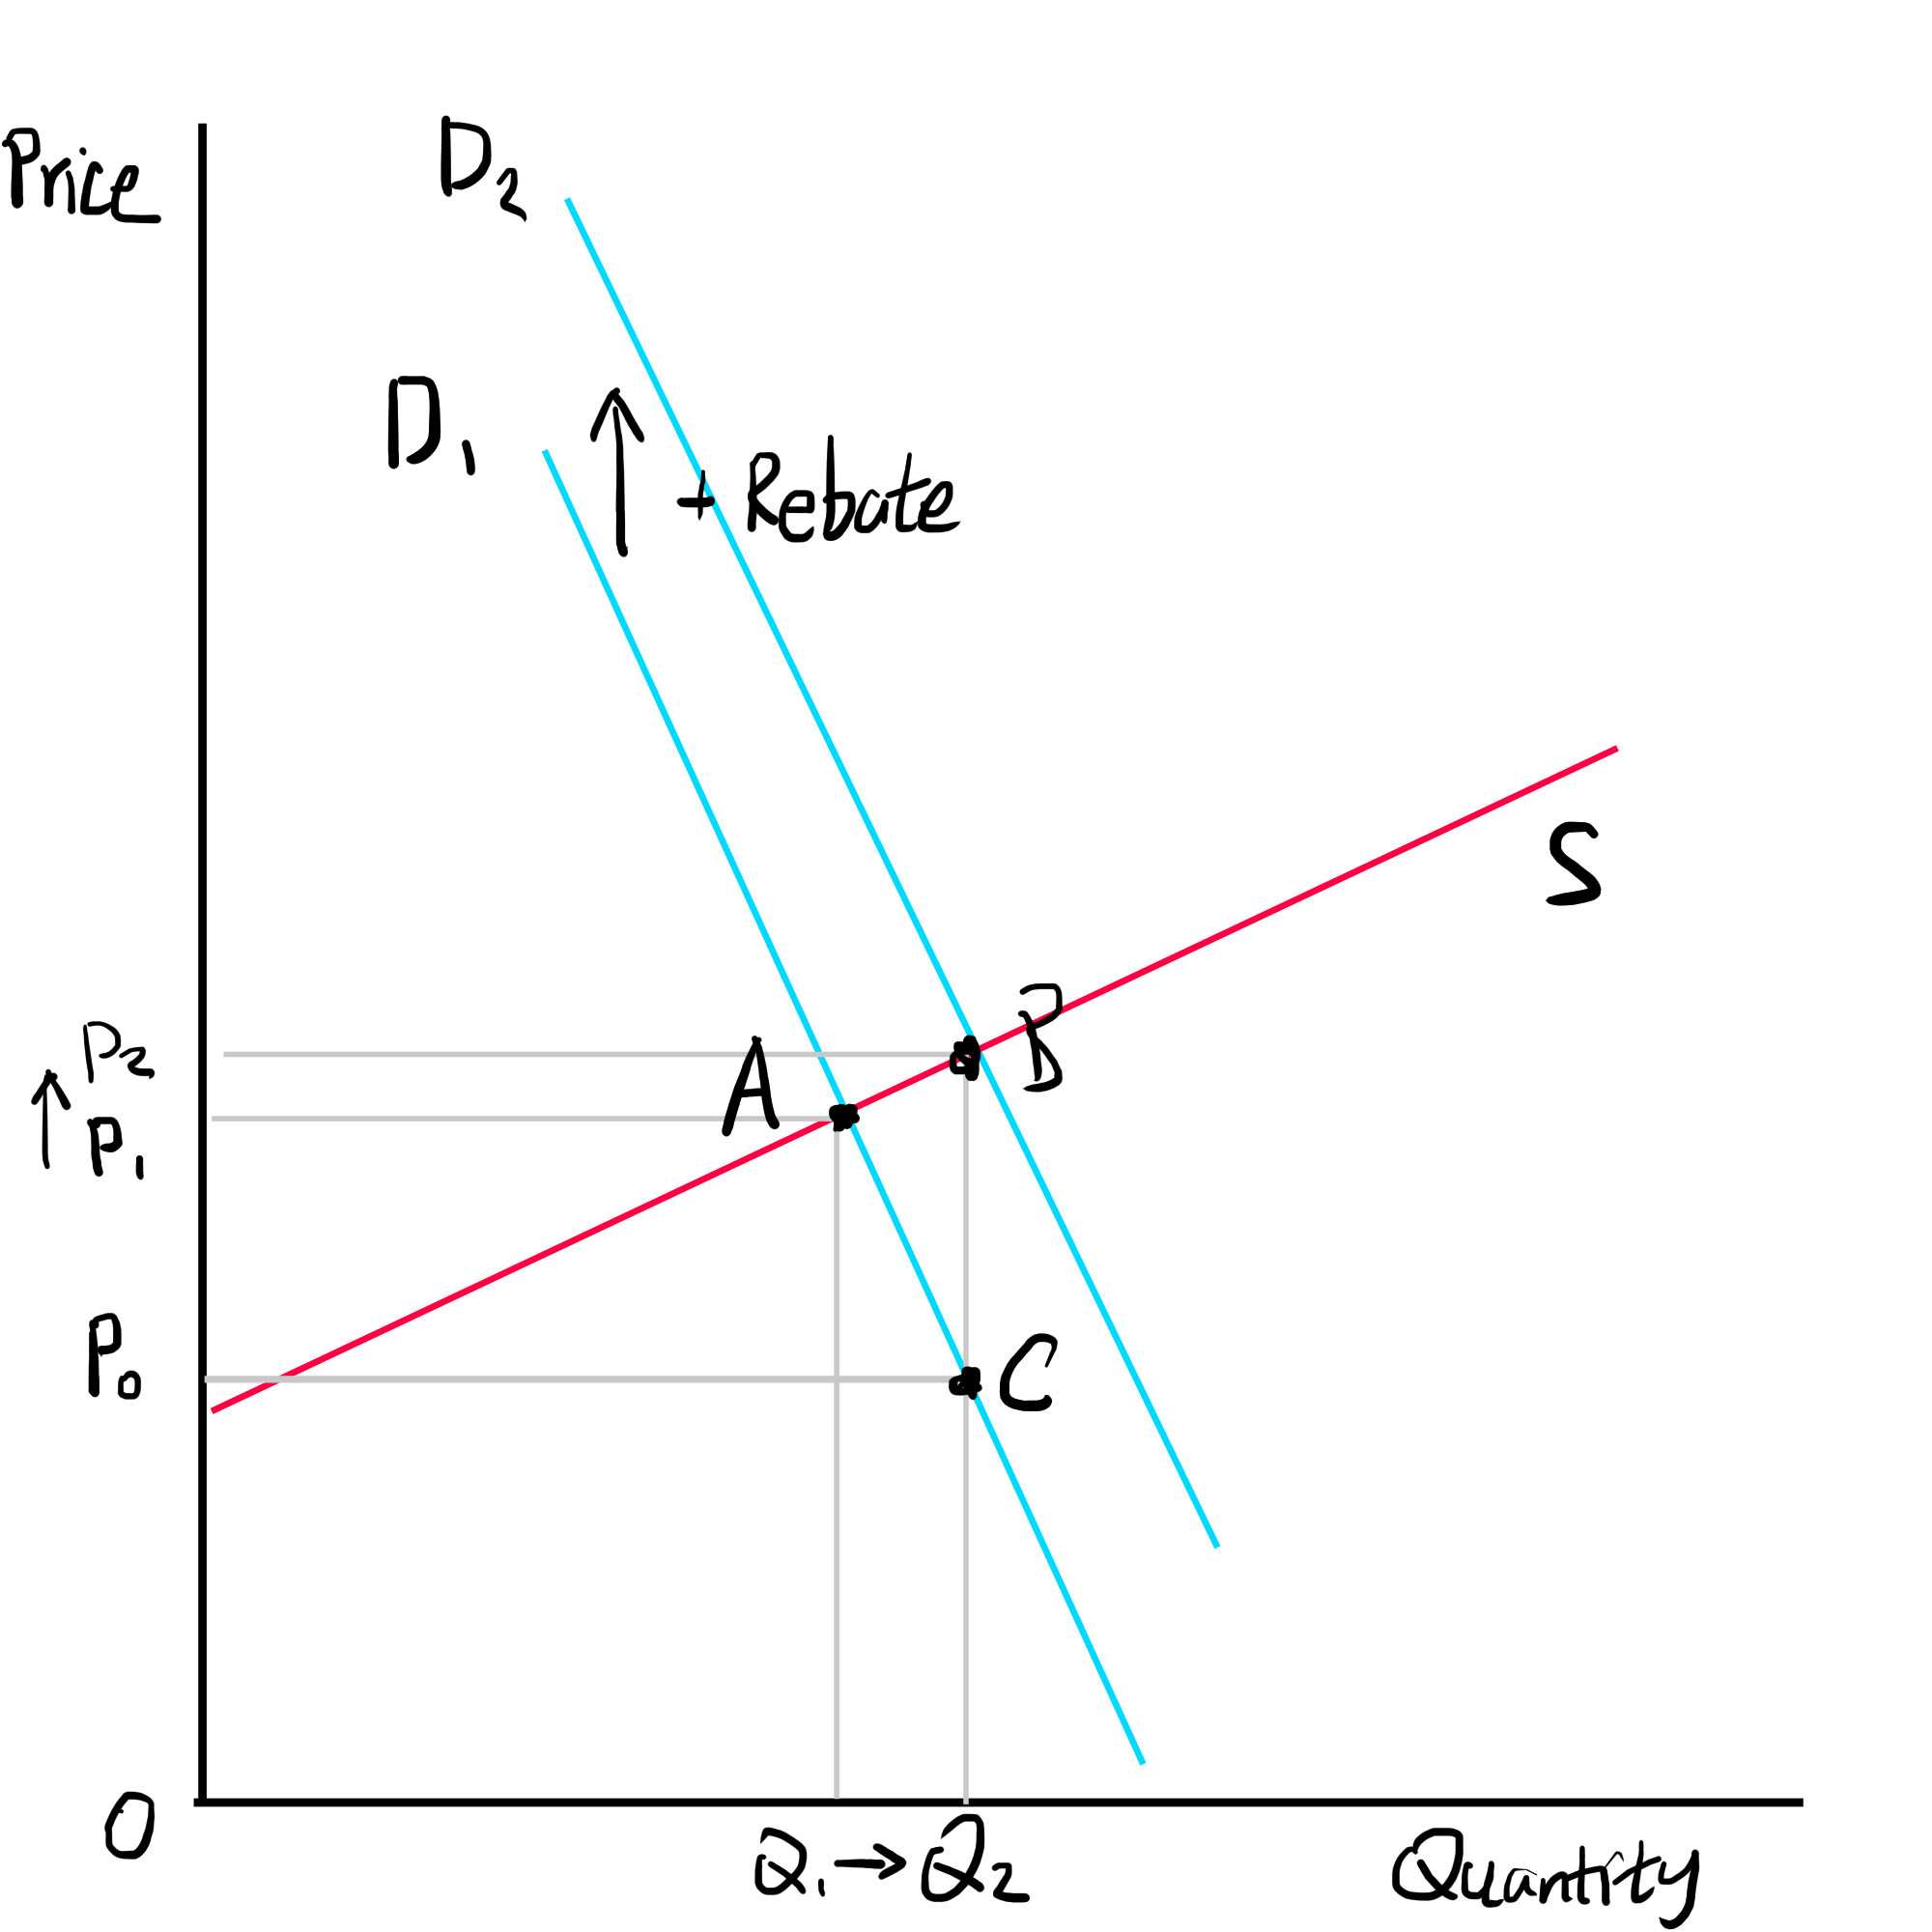
\includegraphics[scale=0.5]{rebate.png}
    \caption{Subsidy on the EV market}
    \label{fig:sub}
\end{figure}

\begin{figure}
    \centering
    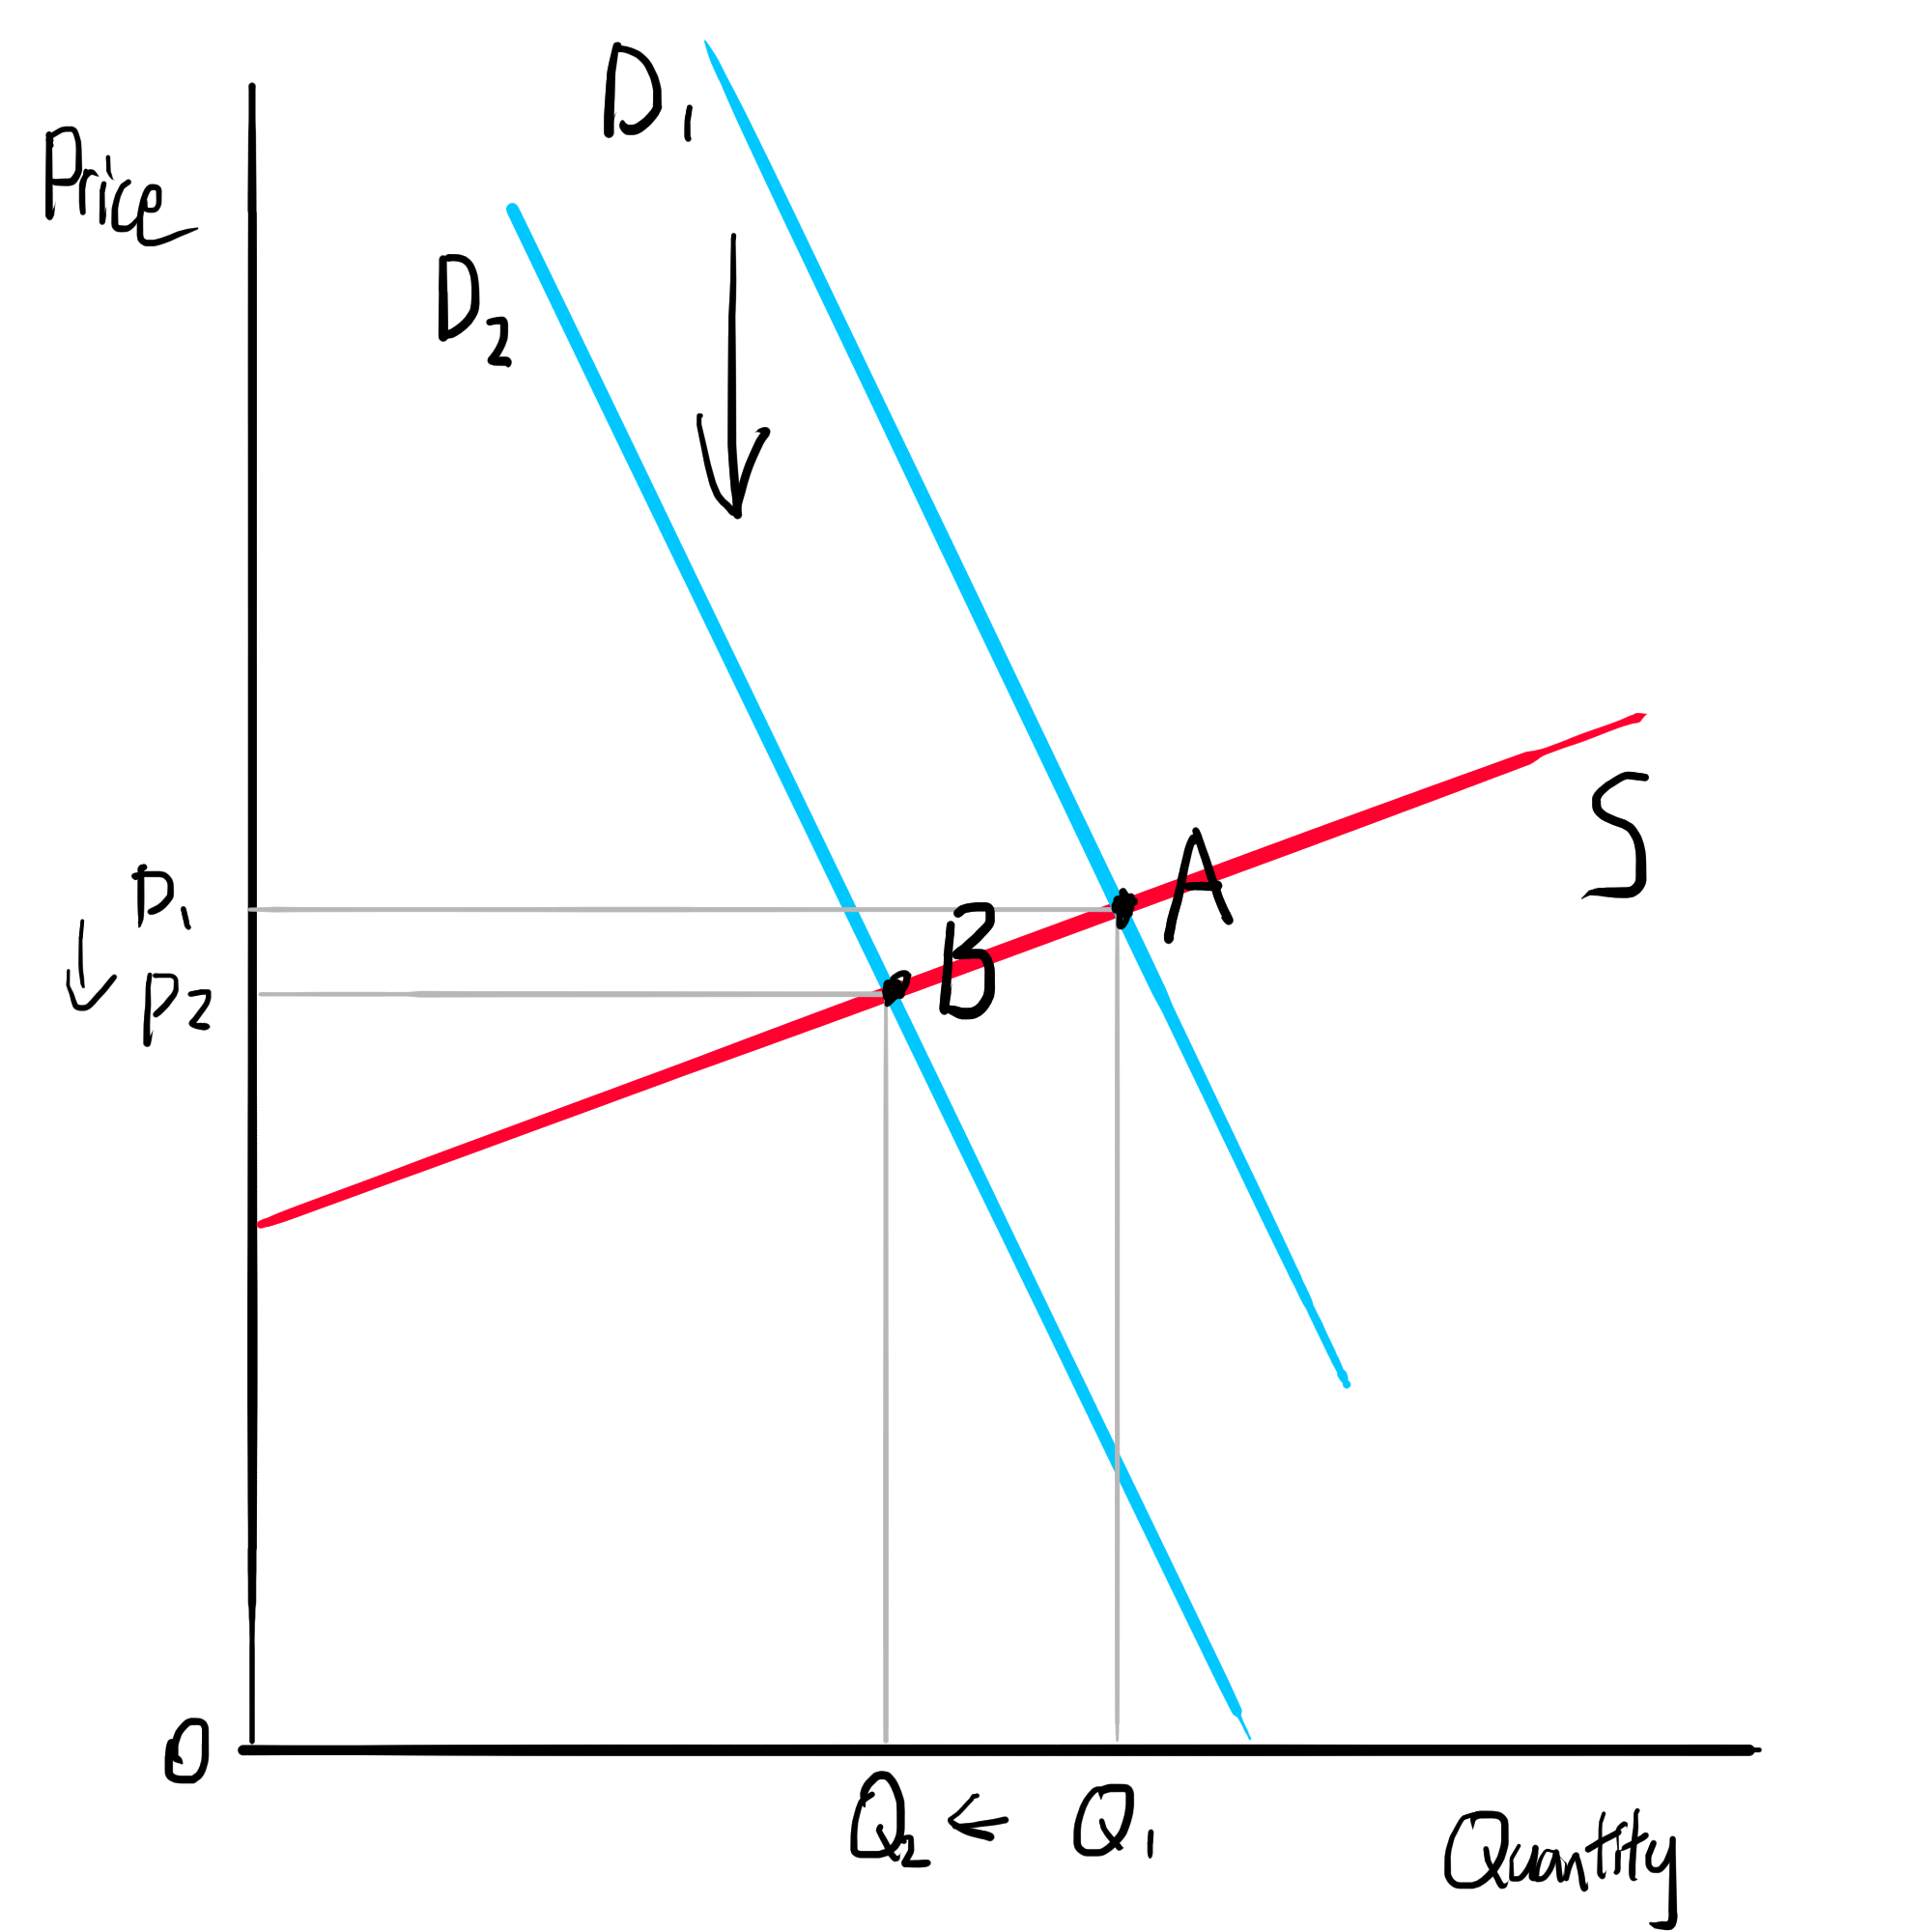
\includegraphics[scale=0.5]{petrol.png}
    \caption{Effect on the petrol vehicle market}
    \label{fig:subpe}
\end{figure}

% percent of income PED
The market of petrol vehicles is impacted by this \textbf{intervention} (figure \ref{fig:subpe}). EVs are substitutes for petrol cars, increase in demand for EVs will shift the demand for gasoline cars to the left from $D_1$ to $D_2$. A surplus is created, with producers lowering the price to clear stock. Market price will decrease from $P_1$ to $P_2$, the quantity demanded of petrol cars will decrease from $Q_1$ to $Q_2$.

%will decrease the cost of production and increase supply from $S_1$ to $S_2$, ceteris parabis. This will create a surplus of electric cars, causing firms to lower their price in order to clear stock --- so to maximize revenue. This causes the equilibrium to shift from point $A$ to point $B$, increasing the quantity consumed from $Q_1$ to $Q_2$ and decreasing the price from $P_1$ to $P_2$. Overall, the subsidy payed by the government is of amount $P_0CBP_2$, and the policy will create a dead-weight loss the size of $ABC$.

% impacts
In the EV market, consumers and producers both benefit from the subsidy: consumer surplus increases by the amount $P_1ACP_0$, producer surplus increases by the amount $P_2BAP_1$. Community surplus will decrease the amount of the DWL.

In the petrol cars market, producers are impacted. Producer surplus will decrease of the amount $P_1ABP_2$, along with a decrease in revenue to $P_2BQ_20$.

The \textbf{intervention} requires a large opportunity cost for the NZ government. The demand curve of EVs is relatively inelastic, for gasoline vehicles are seen to be familiar and safer to existing drivers. This means a large rebate is needed to increase the quantity demanded of EVs. However, because EVs and petrol cars are direct substitutes --- for one can completely replace the other, the cross elasticity of demand (XED) of petrol cars against EVs is high and positive. Therefore even a small change in the price of EVs for consumers will decrease the quantity demanded for petrol cars by a large amount. This means a large opportunity cost is not required to decrease quantity demanded of petrol cars.

\section*{Evaluation}
% long-short term, assumptions, stakeholders, priorities, pros and cons

% effectiveness
The \textbf{intervention} aims to reduce the negative externality of consumption of gasoline vehicles. They emit greenhouse gasses, to which the consumer is not directly paying for, causing a negative externality of consumption --- where the marginal private benefit (MPB) is larger than the marginal social benefit (MSB). The result is an overproduction of petrol cars, figure \ref{fig:extern} illustrates the externality.


\begin{figure}[H]
    \centering
    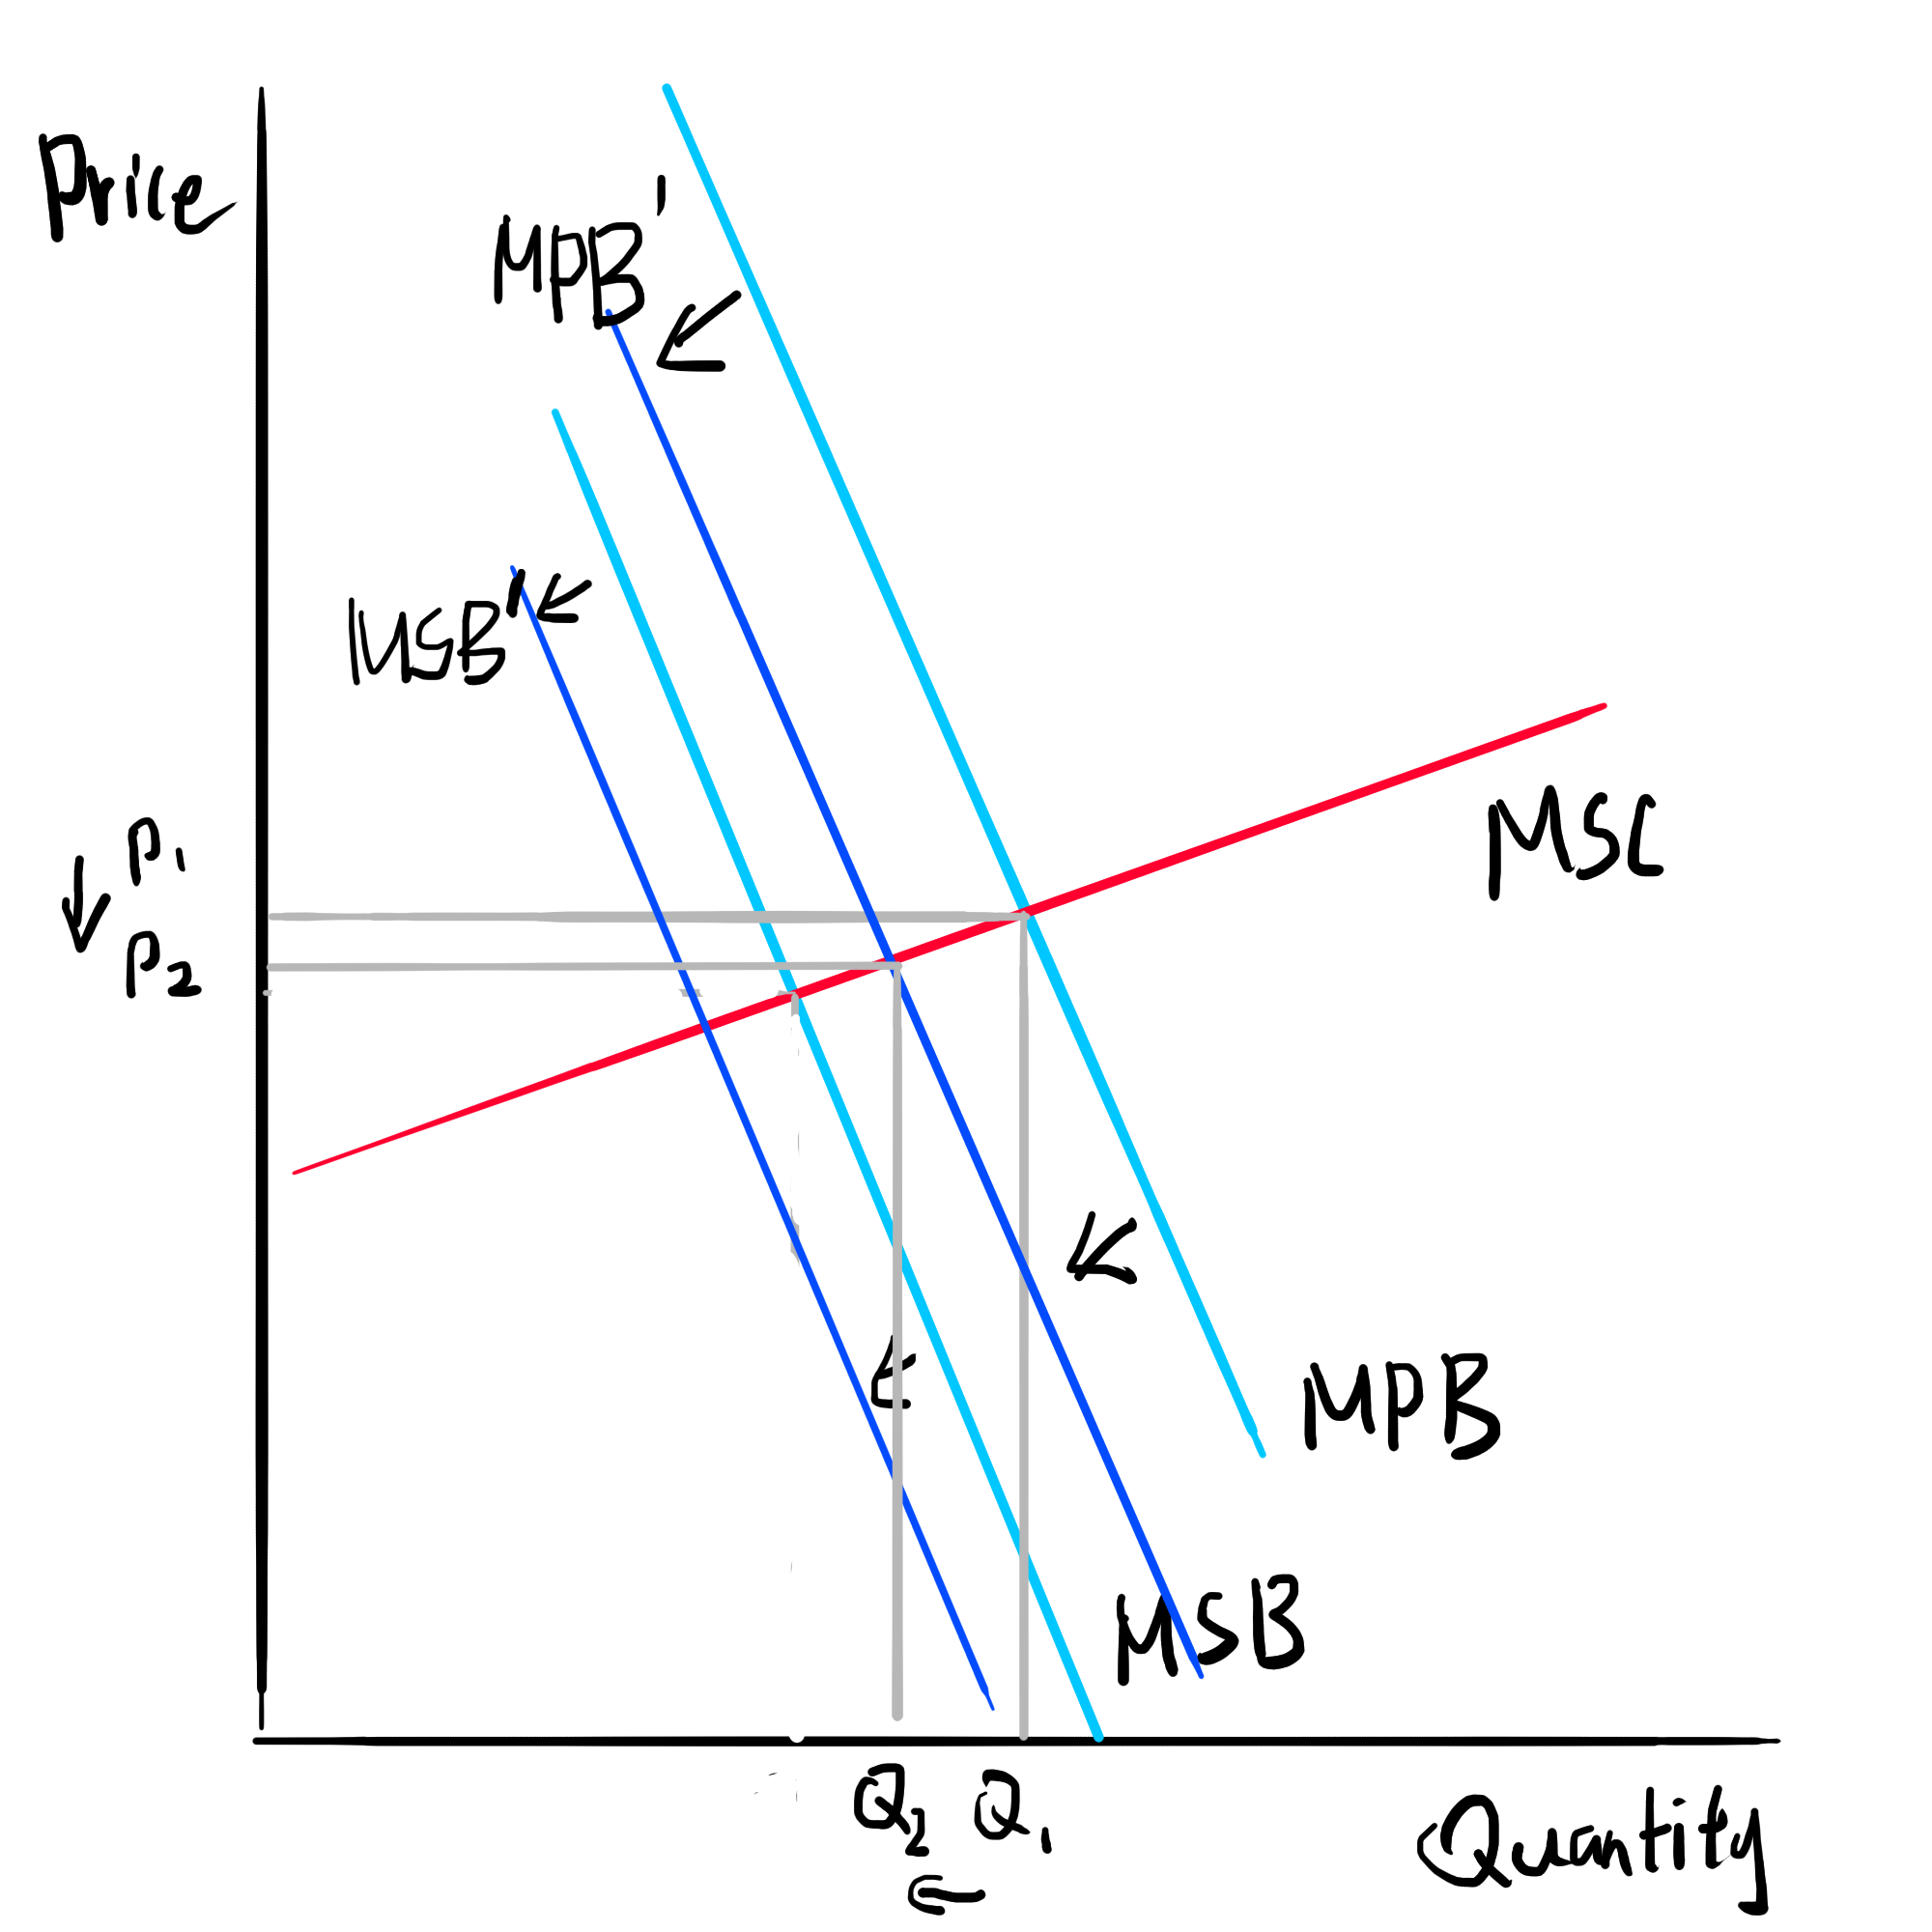
\includegraphics[scale=0.5]{extern_petrol.png}
    \caption{Externality of the petrol car market}
    \label{fig:extern}
\end{figure}

Subsidies in the EV market are effective in reducing this externality. The rebate results in a leftwards shift of the demand of petrol cars, with the large and positive XED ensuring that a small rebate can decrease quantity demanded massively. This largely reduces the overproduction of petrol cars to $Q_2$, and shifts both MSB and MPB leftwards to MSB' and MPB'.

%The subsidy is effective because it increases the quantity of electric cars in the market. Additionally, the intervention decreased EV prices and benefited consumers and producers alike. It is also possible for the lower price to attract consumers currently using petrol cars, and further increasing the quantity of EV consumed. The policy is likely to result in large saturation of EV in the transport market.

Furthermore, reduced emissions will benefit the nation in the long term.
%Positive externalities of consumption occurs when the marginal social benefit (MSB) is higher than the marginal private benefit (MPB) - shown in figure \ref{fig:extern}, so society has a lack of the good of amount $Q_s - Q_1$. The EV subsidy will help reducing the externality by decreasing the marginal social cost, thus increasing the quantity consumed from $Q_1$ to $Q_2$, towards the socially optimal quantity $Q_2$, decreasing market failure.
The reduced externality means that society will benefit as a whole. Decreasing usage of fossil fuels will help the society in reducing damage caused by irregular weather patterns, medical bills of pollution, costs in relocation due to rising sea levels, etc. Everyone benefits from the intervention.

% against
But the \textbf{intervention} may not benefit all equality. The policy mainly affect high-income people who can afford EVs, and unfairly rejects low-income families with taxes on cheaper petrol cars, increasing the cost for the poor. The policy also has opportunity costs, which it can be argued that money could be spent in other areas: transfer payments, building roads and infrastructure etc. --- all of which helps to reduce inequity. Lastly, the subsidy creates a DWL  --- benefits that are lost from the decreased market efficiency.

However, the government had tackled many of these issues. It can allocate unused vehicles from the owners who went electrical to populate the second-hand market, allowing poorer families to afford vehicles; It can extract the money the subsidy requires from taxes in selling new petrol cars. The DWL may be considered insignificant with the mountains of benefits this policy brings.

\section*{Summary}
I agree with New Zealand's \textbf{intervention} in the automobile industry. The policy is effective in reducing externality of petrol cars, increasing climate well-being for all.

\end{document}
